%!TeX program = xelatex
\documentclass[12pt,hyperref,a4paper,UTF8]{ctexart}
\usepackage{USTCReport}
\usepackage{graphicx}
\usepackage{booktabs}
\usepackage{float}
\usepackage{array}
\usepackage{longtable}
\usepackage{fontspec}
\usepackage{setspace}
\usepackage{listings}
\usepackage{hyperref}

\IfFontExistsTF{Times New Roman}{\setmainfont{Times New Roman}}{}
\IfFontExistsTF{SimSun}{\setCJKmainfont{SimSun}}{}
\graphicspath{{figures/}}
\setstretch{1.15}
\setlength{\parindent}{2em}
\setlength{\headheight}{15pt}
\renewcommand{\arraystretch}{1.2}
\lstset{
  language=Python,
  basicstyle=\ttfamily\small,
  breaklines=true,
  columns=fullflexible,
  frame=single,
  showstringspaces=false,
  numbers=left,
  numberstyle=\tiny,
  tabsize=2
}

\title{基于电商用户行为大数据的消费转化漏斗与购买预测分析}
\author{}
\date{\today}

%%-------------------------------正文开始---------------------------%%
\begin{document}

%%-----------------------封面--------------------%%
\cover
\zihao{-4}

%%------------------摘要-------------%%
\begin{abstract}
本文以 Kaggle 公开电商用户行为数据集为研究对象，选取 2019 年 10 月至 12 月三个月全量行为日志，共计 177,493,621 条记录，围绕浏览、加购、购买三个核心行为构建消费转化漏斗，并结合品类、品牌、价格区间和时间维度分析电商消费转化规律。在方法上，本文采用 Python 对 gzip/zip 压缩 CSV 数据进行分块读取，使用 Pandas 和 NumPy 完成数据清洗、聚合统计和特征工程，并使用 Python 图像绘制流程生成可视化结果，最后在抽样用户特征表上使用逻辑回归模型预测用户是否发生购买行为。结果表明，三个月内浏览事件占绝对多数，购买事件为 2,821,836 次；按确定性用户抽样估计，浏览用户到加购用户的转化比例约为 21.79\%，浏览用户到购买用户的转化比例约为 13.31\%。购买预测模型在测试集上取得 89.95\% 的准确率、85.49\% 的召回率和 0.659 的 F1 值，其中加购次数、总行为次数和会话数是识别潜在购买用户的重要变量。研究说明，大规模行为日志能够为电商平台的转化诊断、品类运营和用户分层营销提供数据支持。

\textbf{关键词：} 电商大数据；用户行为；转化漏斗；购买预测；逻辑回归；Python
\end{abstract}

\thispagestyle{empty}

%%------------------------正文页从这里开始-------------------%
\newpage
\tableofcontents
\newpage

\section{研究背景与问题提出}

随着平台经济和在线零售的发展，电商平台沉淀了大量用户行为日志。与传统问卷或抽样交易数据相比，行为日志具有规模大、频率高、时间连续、路径完整等特征，能够刻画用户从商品曝光、浏览、加购到最终购买的全过程。对于平台经营者而言，理解用户在哪些环节流失、哪些品类和品牌贡献主要销售额、哪些行为信号能够预示购买，是提升转化效率和优化运营策略的重要基础。

本课程强调使用 Python 语言及其数据分析生态处理经济数据，并将采集、清洗、分析、可视化和机器学习方法落地到实际案例。基于这一要求，本文选择电商用户行为数据作为案例，一方面该数据具备典型的经济管理含义，能够对应消费者决策、促销活动和平台运营；另一方面，原始数据达到亿级记录，适合展示分块处理、聚合计算和机器学习建模等大数据分析流程。

本文围绕三个问题展开：
\begin{enumerate}
  \item 三个月电商用户行为在浏览、加购、购买三个阶段上的总体结构如何？
  \item 2019 年 10 月、11 月、12 月之间的行为规模和转化效率是否存在明显差异？
  \item 能否利用用户历史行为特征预测其是否发生购买，从而支持潜在消费者识别？
\end{enumerate}

\section{研究设计与指标体系}

\subsection{业务链路拆解}

电商消费行为通常不是一次性完成的，而是由多个连续环节构成。用户首先通过搜索、推荐或活动入口接触商品，随后进入商品详情页形成浏览记录；当用户对商品产生更强兴趣时，可能将商品加入购物车；最终，只有部分用户完成支付并形成购买记录。因此，本文将平台消费过程抽象为“浏览--加购--购买”的三阶段漏斗。

这一抽象虽然简化了真实平台中收藏、搜索、优惠券领取、客服咨询等行为，但能够覆盖本数据集中最重要的三类事件，并且便于将统计分析与业务动作对应起来。浏览阶段主要反映流量规模和商品曝光，加购阶段反映初步购买意向，购买阶段反映最终交易结果。若浏览量很高但加购率较低，问题更可能出现在商品匹配、价格吸引力或详情页信息；若加购量很高但购买率较低，则问题更可能出现在价格比较、库存、配送、支付体验或促销机制。

\subsection{指标设计}

为了避免只停留在描述性统计，本文从规模、转化、结构和预测四个层面设计指标。规模指标回答“有多少行为”，转化指标回答“行为如何向交易推进”，结构指标回答“哪些商品和价格段贡献交易”，预测指标回答“能否识别潜在购买用户”。具体指标如下表所示。

\begin{table}[H]
\centering
\caption{本文指标体系}
\begin{tabular}{p{0.18\textwidth}p{0.30\textwidth}p{0.42\textwidth}}
\toprule
指标层面 & 代表指标 & 解释目的 \\
\midrule
规模指标 & 浏览数、加购数、购买数、购买金额 & 衡量平台整体活跃度和交易规模 \\
转化指标 & 浏览到加购比例、浏览到购买比例、加购到购买比例 & 判断用户在哪个环节出现主要流失 \\
结构指标 & 品类销售额、品牌销售额、价格区间销售额 & 识别主要交易来源和商品结构特征 \\
时间指标 & 日度事件数、月度事件数、小时峰值 & 观察促销季、年末消费和日内行为节奏 \\
预测指标 & Accuracy、Precision、Recall、F1、特征系数 & 评估机器学习模型是否可用于用户分层 \\
\bottomrule
\end{tabular}
\end{table}

\subsection{分析假设}

本文的分析基于三个业务假设。第一，用户行为强度越高，购买概率通常越高；但行为范围过宽可能意味着用户仍在比较，购买意愿未必确定。第二，加购行为比单纯浏览更能代表明确购买意向，因此在预测模型中应当具有更强解释力。第三，促销期会显著抬升流量和加购规模，但转化效率是否同步提升需要通过购买率单独检验。

后文的统计和建模结果将围绕这些假设展开。如果结果支持假设，则说明行为日志可以为平台运营提供可解释信号；如果结果不支持，则需要反思指标设计或进一步引入更细粒度的价格、优惠、库存和推荐位数据。

\section{数据来源与处理流程}

\subsection{数据来源}

本文使用 Kaggle 数据集 ``E-commerce behavior data from multi category store''。原始数据为多品类电商平台用户行为日志，字段包括事件时间、事件类型、商品编号、品类编号、品类名称、品牌、价格、用户编号和会话编号等。本文选取 2019 年 10 月、11 月、12 月三个月数据，文件形态包括 \texttt{.csv.gz} 与 \texttt{.csv.zip} 压缩文件。

三个月数据的总处理记录数为 177,493,621 条。由于单月 CSV 解压后体积较大，本文没有将压缩文件一次性完全解压，而是采用 Pandas 的 \texttt{read\_csv(chunksize=...)} 按百万行分块读取。这一方式能够将内存占用控制在可接受范围内，同时保留全量数据的统计信息。

\subsection{字段处理与特征构造}

原始字段经过如下处理：
\begin{itemize}
  \item 将 \texttt{event\_time} 转换为时间类型，并提取日期、小时和月份字段；
  \item 将 \texttt{event\_type} 映射为浏览、加购、购买三个行为指标；
  \item 对价格字段进行数值化处理，并按照价格区间统计不同价位商品的转化情况；
  \item 对缺失品牌和品类名称统一填充为 \texttt{unknown}，避免分组统计时丢失记录；
  \item 基于用户编号进行确定性抽样，构造用户级特征表用于机器学习建模。
\end{itemize}

在建模数据中，本文以用户-月份为观察单位，构造总行为次数、浏览次数、加购次数、访问会话数、活跃天数、浏览商品数、浏览品类数、浏览品牌数、平均价格和最高价格等变量，并以当月是否发生购买作为二分类标签。

\subsection{技术路线}

本文的技术路线包括四个环节：第一，分块读取三个月压缩行为日志；第二，对事件、日期、月份、小时、品类、品牌和价格区间进行聚合；第三，构造用户级机器学习样本并训练逻辑回归模型；第四，生成图表并完成报告与展示材料。

\subsection{数据口径与质量控制}

本文的数据口径分为事件口径与用户口径两类。事件口径直接统计日志中的每条行为记录，适合衡量浏览量、加购量、购买量和销售额；用户口径需要对 \texttt{user\_id} 去重，适合构造转化漏斗和用户级预测样本。由于三个月数据规模较大，事件总量采用全量统计，唯一用户漏斗采用确定性抽样估计。这样既保留了全量事件规模，又避免在本地环境中维护过大的用户集合。

数据清洗主要处理四类问题。第一，时间字段统一解析为日期、小时和月份，保证跨文件聚合时口径一致。第二，缺失品牌和品类统一填充为 \texttt{unknown}，避免分组时丢失记录。第三，价格字段转为数值型并将缺失值置为 0，用于购买金额和价格区间统计。第四，用户会话缺失值统一填充，保证会话数统计不会因空值被忽略。

\begin{lstlisting}[caption={分块读取与核心字段清洗示例}]
usecols = [
    "event_time", "event_type", "product_id", "category_id",
    "category_code", "brand", "price", "user_id", "user_session"
]

reader = pd.read_csv(file_path, usecols=usecols,
                     chunksize=1_000_000, compression="infer")

for chunk in reader:
    chunk["event_time"] = pd.to_datetime(
        chunk["event_time"], utc=True, errors="coerce"
    )
    chunk = chunk.dropna(subset=["event_time"])
    chunk["date"] = chunk["event_time"].dt.strftime("%Y-%m-%d")
    chunk["hour"] = chunk["event_time"].dt.hour
    chunk["month"] = chunk["date"].str.slice(0, 7)
    chunk["price"] = pd.to_numeric(chunk["price"], errors="coerce").fillna(0)
\end{lstlisting}

上述代码体现了本案例处理大文件的核心思路：每次只读入 100 万行，将清洗、字段派生和聚合统计放在同一个循环中完成。处理完一个分块后，只保留小规模聚合结果和用户抽样特征，而不是长期保存原始明细数据。

\subsection{聚合计算与可复现性}

为了保证结果可复现，本文所有统计表均由同一套脚本生成，并输出到 \texttt{data/processed/ecommerce} 目录。主要结果包括事件类型汇总、日度行为汇总、月度行为汇总、价格区间汇总、品类汇总、品牌汇总、转化漏斗和用户特征样本。用户抽样采用固定规则 \texttt{user\_id \% 40 == 0}，因此每次运行都会得到相同的样本集合。

\begin{lstlisting}[caption={按行为类型和月份聚合的代码示例}]
chunk["is_view"] = (chunk["event_type"] == "view").astype("int8")
chunk["is_cart"] = (chunk["event_type"] == "cart").astype("int8")
chunk["is_purchase"] = (chunk["event_type"] == "purchase").astype("int8")
chunk["revenue"] = np.where(
    chunk["event_type"] == "purchase", chunk["price"], 0.0
)

month_part = (
    chunk.groupby(["month", "event_type"], as_index=False)
         .agg(events=("event_type", "size"),
              users_chunk_sum=("user_id", "nunique"),
              revenue=("revenue", "sum"))
)
\end{lstlisting}

在解释结果时需要注意，\texttt{users\_chunk\_sum} 是分块内唯一用户数的加总，可能重复计算跨分块出现的同一用户，因此只用于辅助判断用户参与规模，不作为严格唯一用户数。严格漏斗分析使用确定性抽样用户集合估计，这一点在后文单独说明。

\section{总体行为结构分析}

\subsection{事件类型分布}

三个月数据中，浏览、加购和购买事件的数量差异明显。浏览事件为 167,321,576 次，加购事件为 7,350,209 次，购买事件为 2,821,836 次。浏览行为占据绝对主体，说明大多数用户行为停留在商品信息获取和比较阶段，只有较少比例最终进入购物车和支付环节。

\begin{table}[H]
\centering
\caption{三个月用户行为事件汇总}
\begin{tabular}{lrrr}
\toprule
事件类型 & 事件数 & 分块用户数汇总 & 购买金额 \\
\midrule
浏览 view & 167,321,576 & 27,462,005 & 0.00 \\
加购 cart & 7,350,209 & 3,551,284 & 0.00 \\
购买 purchase & 2,821,836 & 2,053,387 & 849,329,221.91 \\
\bottomrule
\end{tabular}
\end{table}

\begin{figure}[H]
\centering
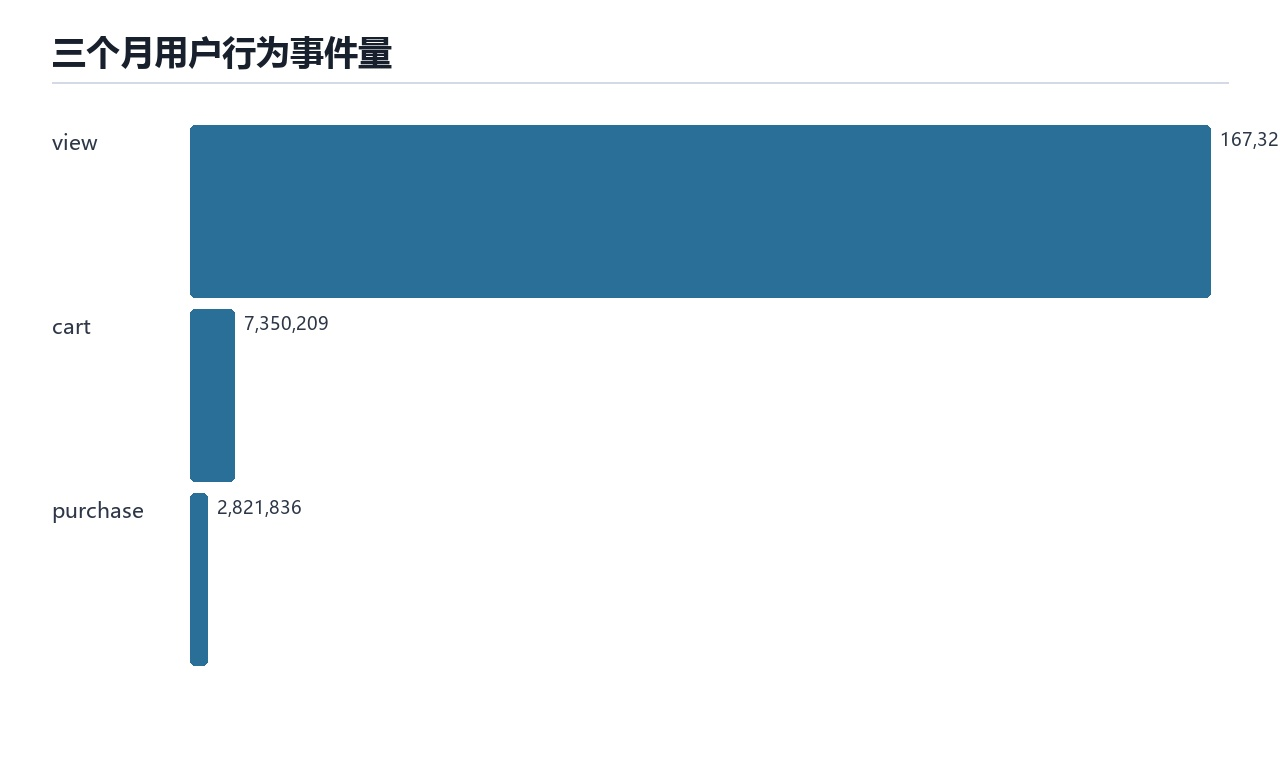
\includegraphics[width=0.92\textwidth]{event_type_summary.jpg}
\caption{三个月用户行为事件量}
\end{figure}

从事件结构看，浏览到加购、加购到购买之间存在明显漏斗衰减。对平台而言，单纯扩大流量并不一定带来等比例的交易增长，关键在于提升商品匹配、价格吸引力、库存可得性和支付流程效率。

\subsection{月度变化}

按月份观察，2019 年 10 月购买事件为 742,849 次，11 月为 916,939 次，12 月为 1,162,048 次。11 月和 12 月的购买规模明显高于 10 月，反映促销季和年末消费需求对电商转化的拉动作用。

\begin{table}[H]
\centering
\caption{各月行为事件数量}
\begin{tabular}{lrrr}
\toprule
月份 & 浏览 & 加购 & 购买 \\
\midrule
2019-10 & 40,779,399 & 926,516 & 742,849 \\
2019-11 & 63,556,110 & 3,028,930 & 916,939 \\
2019-12 & 62,986,067 & 3,394,763 & 1,162,048 \\
\bottomrule
\end{tabular}
\end{table}

\begin{figure}[H]
\centering
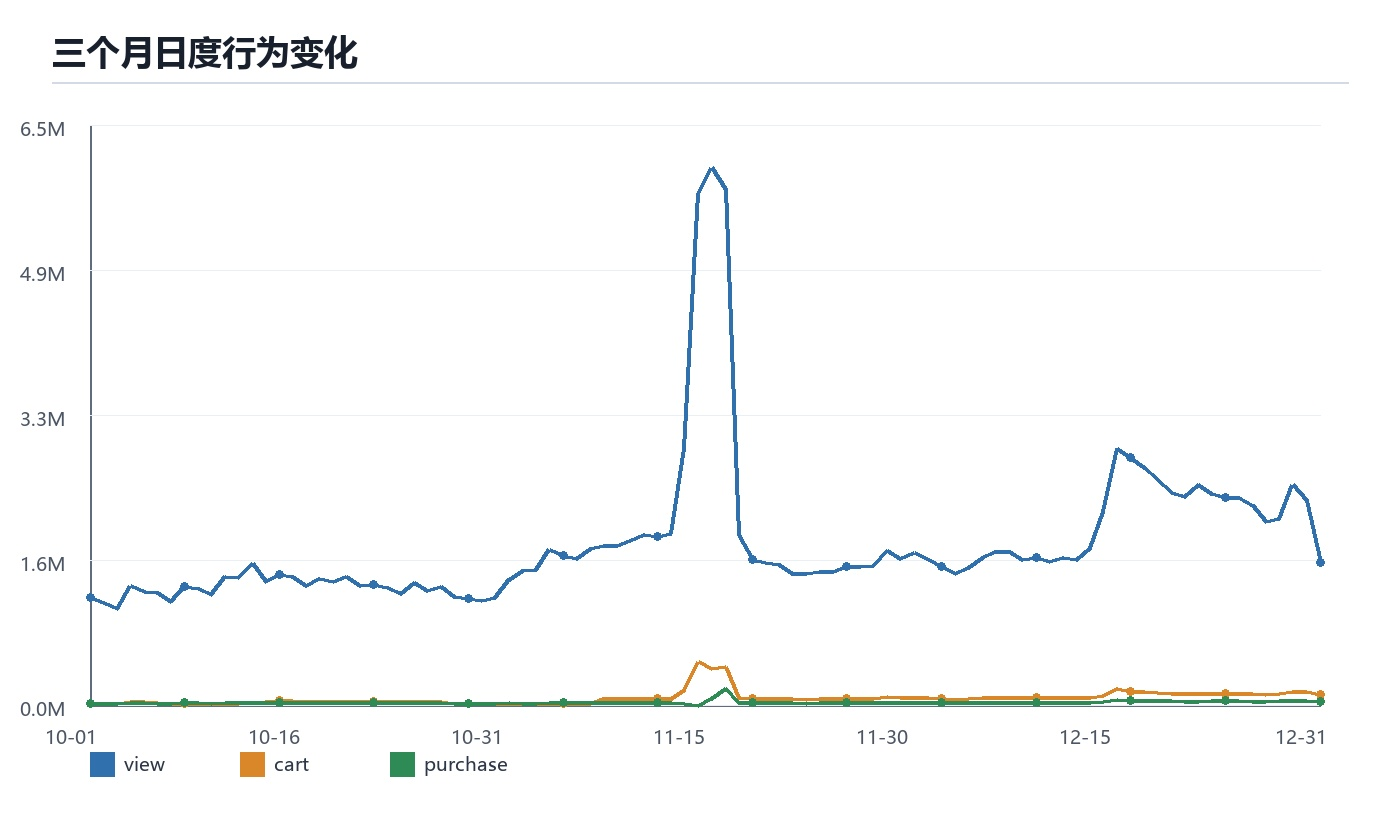
\includegraphics[width=0.96\textwidth]{daily_events.jpg}
\caption{三个月日度行为变化}
\end{figure}

\begin{figure}[H]
\centering
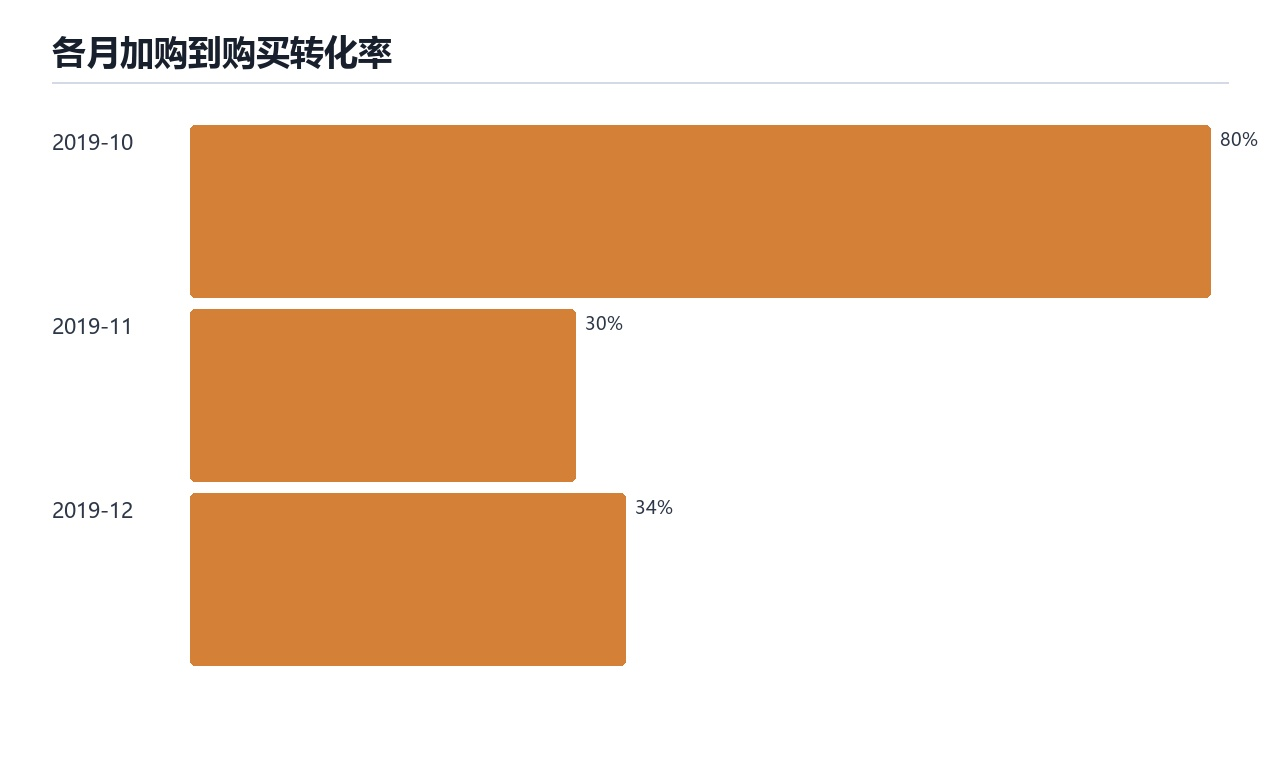
\includegraphics[width=0.86\textwidth]{monthly_cart_purchase_rate.jpg}
\caption{各月加购到购买转化率}
\end{figure}

月度数据说明，11 月的浏览和加购规模显著扩大，但加购到购买的转化效率并未同步上升；12 月购买事件进一步增加，说明年末消费场景可能带来更强的实际支付意愿。由此可以看出，促销月不仅需要关注流量峰值，也需要关注购物车沉淀后的支付转化。

\subsection{小时维度观察}

从小时维度看，不同行为的峰值时间并不完全一致。浏览事件峰值出现在 16 点，峰值事件数为 11,564,432；加购事件峰值出现在 8 点，峰值事件数为 495,343；购买事件峰值出现在 9 点，峰值事件数为 211,140。该现象说明，用户的信息搜索、购物车整理和支付行为可能发生在不同时间段，平台运营可以将推荐曝光、购物车提醒和支付激励放在不同触达时点。

\begin{table}[H]
\centering
\caption{不同行为的小时峰值}
\begin{tabular}{lrr}
\toprule
行为类型 & 峰值小时 & 峰值事件数 \\
\midrule
浏览 view & 16 & 11,564,432 \\
加购 cart & 8 & 495,343 \\
购买 purchase & 9 & 211,140 \\
\bottomrule
\end{tabular}
\end{table}

这一结果也提醒，单纯以日为单位观察促销效果可能掩盖用户在一天内的行为节奏。更细的小时级分析可以支持分时段投放、首页资源位调整和购物车召回策略。

\section{转化漏斗分析}

本文使用用户编号的确定性抽样估计唯一用户漏斗规模。抽样方法为按 \texttt{user\_id} 取模抽样，抽样比例约为 1/40，并将样本唯一用户数放大到总体估计。该方法不会影响事件总量统计，但唯一用户数属于估计值。

\begin{table}[H]
\centering
\caption{用户转化漏斗估计结果}
\begin{tabular}{lrrr}
\toprule
阶段 & 样本唯一用户数 & 估计唯一用户数 & 相对浏览用户比例 \\
\midrule
浏览 & 196,347 & 7,853,880 & 100.00\% \\
加购 & 42,791 & 1,711,640 & 21.79\% \\
购买 & 26,142 & 1,045,680 & 13.31\% \\
\bottomrule
\end{tabular}
\end{table}

\begin{figure}[H]
\centering
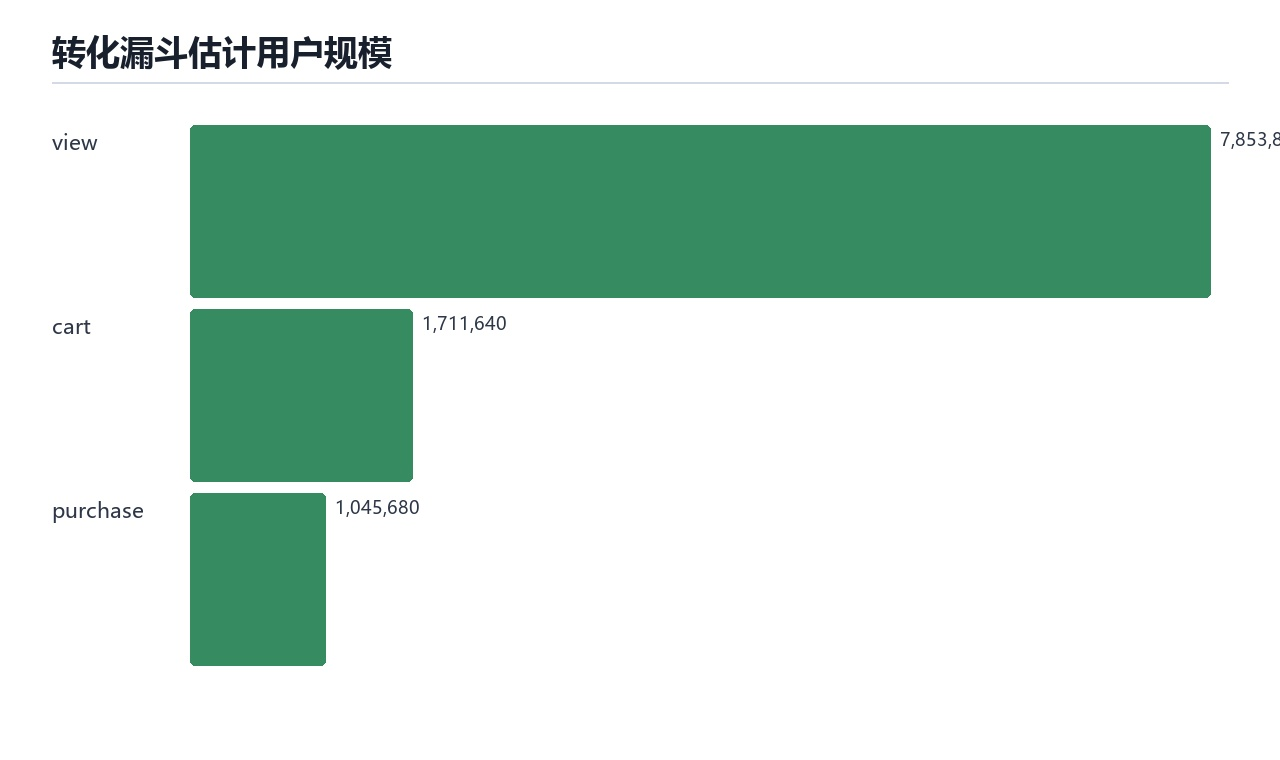
\includegraphics[width=0.86\textwidth]{funnel_users.jpg}
\caption{转化漏斗估计用户规模}
\end{figure}

漏斗结果显示，约五分之一的浏览用户进入加购阶段，约八分之一的浏览用户最终发生购买。加购用户与购买用户之间仍存在显著流失，这部分用户通常已经表现出较高意愿，适合通过价格提醒、优惠券、库存提示、免邮门槛和个性化推荐等方式进行二次触达。

\section{品类、品牌与价格结构}

\subsection{品类贡献}

从销售额看，手机、灯具工具、耳机、钟表、电视、冰箱、洗衣机等品类贡献较高。其中 \texttt{electronics.smartphone} 的购买次数为 729,644 次，销售额约 338,105,371.98；\texttt{construction.tools.light} 的购买次数为 502,274 次，销售额约 215,188,124.66。

\begin{table}[H]
\centering
\caption{销售额最高的品类 Top 8}
\begin{tabular}{lrr}
\toprule
品类 & 购买次数 & 销售额 \\
\midrule
electronics.smartphone & 729,644 & 338,105,371.98 \\
construction.tools.light & 502,274 & 215,188,124.66 \\
unknown & 495,659 & 62,608,388.30 \\
electronics.audio.headphone & 90,224 & 18,763,126.58 \\
electronics.clocks & 78,783 & 20,744,277.17 \\
sport.bicycle & 60,124 & 8,275,757.66 \\
electronics.video.tv & 56,767 & 21,868,719.93 \\
appliances.kitchen.refrigerators & 56,060 & 24,812,288.76 \\
\bottomrule
\end{tabular}
\end{table}

\begin{figure}[H]
\centering
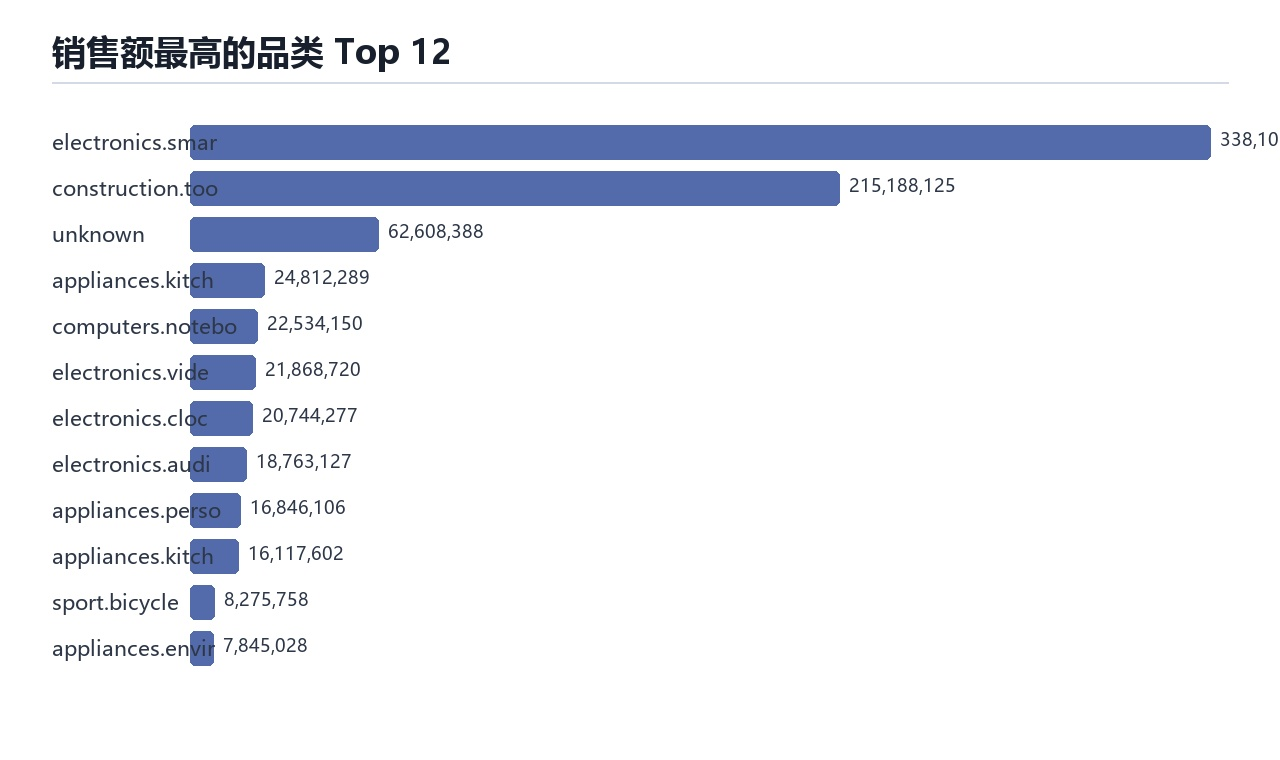
\includegraphics[width=0.96\textwidth]{top_categories_revenue.jpg}
\caption{销售额最高的品类 Top 12}
\end{figure}

\subsection{品牌贡献}

品牌维度上，Apple、Samsung、Xiaomi、Huawei 等消费电子品牌具有较强交易贡献。Apple 的购买次数为 518,449 次，但销售额达到 396,118,468.60，说明其客单价较高；Samsung 的购买次数为 638,864 次，销售额为 173,136,224.53，表现出更高的交易频次。

\begin{figure}[H]
\centering
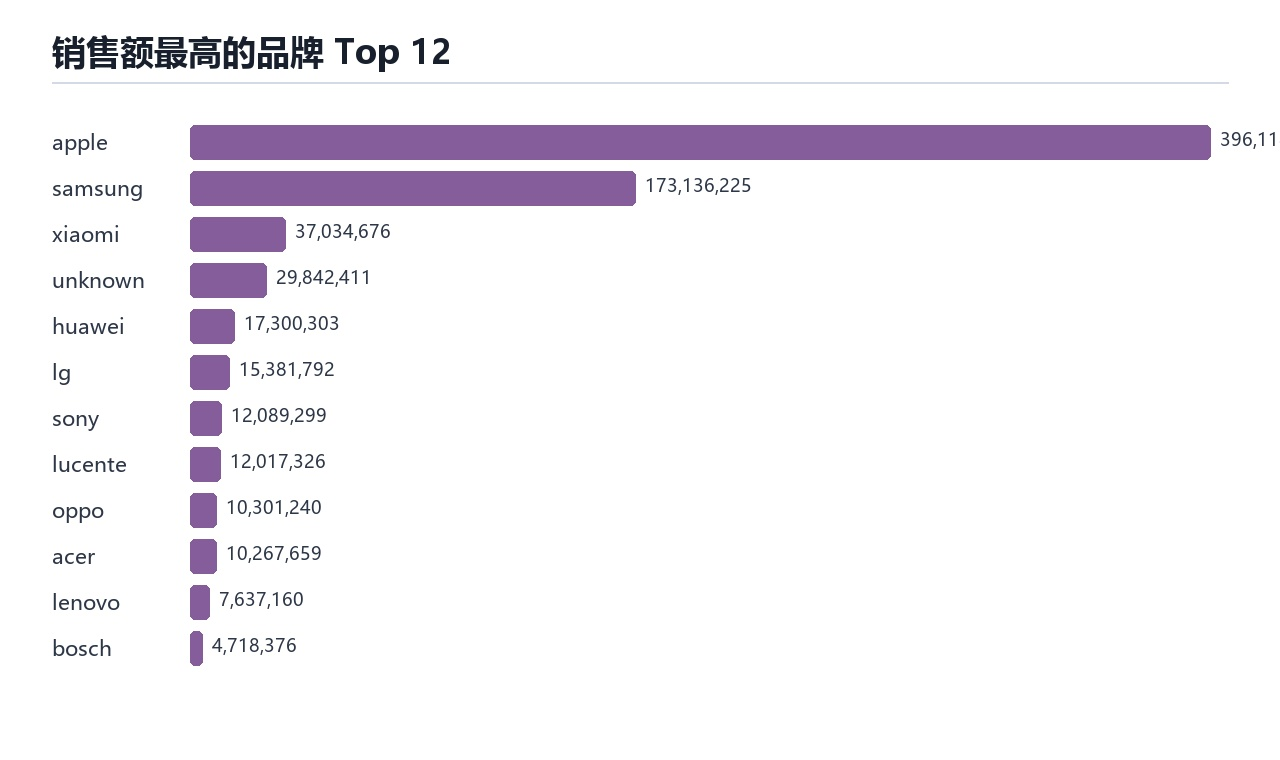
\includegraphics[width=0.96\textwidth]{top_brands_revenue.jpg}
\caption{销售额最高的品牌 Top 12}
\end{figure}

\subsection{价格区间}

价格区间统计显示，200--500、500--1000 和 1000--5000 价格段贡献了主要销售额。其中 500--1000 价格段购买金额约 268,103,353.39，200--500 价格段约 233,270,380.69，1000--5000 价格段约 194,988,617.34。相比低价商品，高价商品即使购买次数较少，也能贡献较高销售额。

\begin{table}[H]
\centering
\caption{购买金额最高的价格区间}
\begin{tabular}{lrrr}
\toprule
价格区间 & 购买事件数 & 购买金额 & 金额占比 \\
\midrule
500--1000 & 357,384 & 268,103,353.39 & 31.57\% \\
200--500 & 749,264 & 233,270,380.69 & 27.47\% \\
1000--5000 & 144,734 & 194,988,617.34 & 22.96\% \\
100--200 & 767,009 & 113,879,642.68 & 13.41\% \\
50--100 & 353,637 & 25,785,305.73 & 3.04\% \\
10--50 & 403,248 & 12,994,502.71 & 1.53\% \\
0--10 & 46,560 & 307,419.37 & 0.04\% \\
\bottomrule
\end{tabular}
\end{table}

从价格结构看，购买次数最多的区间并不一定贡献最高销售额。100--200 和 200--500 价格段购买次数较高，说明中低价位商品具备较强交易频次；500--1000 和 1000--5000 价格段虽然购买次数较少，但金额贡献更大。对平台而言，低价商品适合承担引流和高频复购功能，高价商品则需要更重视商品详情、品牌信任和售后保障。

\section{购买预测模型}

\subsection{模型设定}

为了体现机器学习方法在电商运营中的应用，本文构建用户购买预测模型。模型以用户-月份为样本单位，标签为用户当月是否发生购买，特征包括总行为次数、浏览次数、加购次数、访问会话数、活跃天数、浏览商品数、浏览品类数、浏览品牌数、平均价格和最高价格。模型采用逻辑回归，其基本形式为：

\[
P(y=1|x)=\frac{1}{1+\exp[-(\beta_0+\beta_1x_1+\cdots+\beta_kx_k)]}
\]

其中，\(y=1\) 表示用户发生购买，\(x\) 为用户行为特征。由于正负样本不平衡，训练过程中对正样本设置较高权重，并在测试集上选择使 F1 值较优的分类阈值。

\subsection{标签口径与样本构造}

本文的建模样本以“用户-月份”为单位，而不是以单条事件为单位。这样处理有两个原因。第一，单条事件难以表达用户在一个阶段内的累积兴趣，浏览一次、浏览十次和多次加购在购买意愿上显然不同。第二，用户级特征更接近实际运营中的人群分层场景，平台通常需要判断某个用户是否值得触达，而不是判断某一条浏览日志是否会转化。

标签定义为：若用户在某个月内至少发生一次购买事件，则该用户-月份样本的 \texttt{converted} 取值为 1，否则为 0。需要说明的是，该标签并非严格的实时预测标签，因为当月后续行为可能已经包含购买后的活动。为了避免夸大模型能力，本文在结论中将其定位为“用户购买倾向识别”而非“实时下单预测”。如果要进一步提升严谨性，可以将每月前若干天行为作为特征，将后若干天是否购买作为标签，形成时间前后严格分离的滚动预测任务。

特征构造时，本文对用户当月行为进行聚合，包括总事件数、浏览次数、加购次数、访问会话数、活跃天数、浏览商品数、浏览品类数、浏览品牌数、平均价格和最高价格。这些变量分别对应活跃程度、购买意向、兴趣集中度和价格偏好。

\subsection{模型结果}

模型使用 249,999 条抽样用户-月份记录，其中训练集 199,999 条，测试集 50,000 条。测试集结果如表所示。

\begin{table}[H]
\centering
\caption{购买预测模型评估结果}
\begin{tabular}{lr}
\toprule
指标 & 数值 \\
\midrule
正样本比例 & 11.43\% \\
分类阈值 & 0.525 \\
准确率 Accuracy & 89.95\% \\
精确率 Precision & 53.68\% \\
召回率 Recall & 85.49\% \\
F1 值 & 0.659 \\
\bottomrule
\end{tabular}
\end{table}

\begin{figure}[H]
\centering
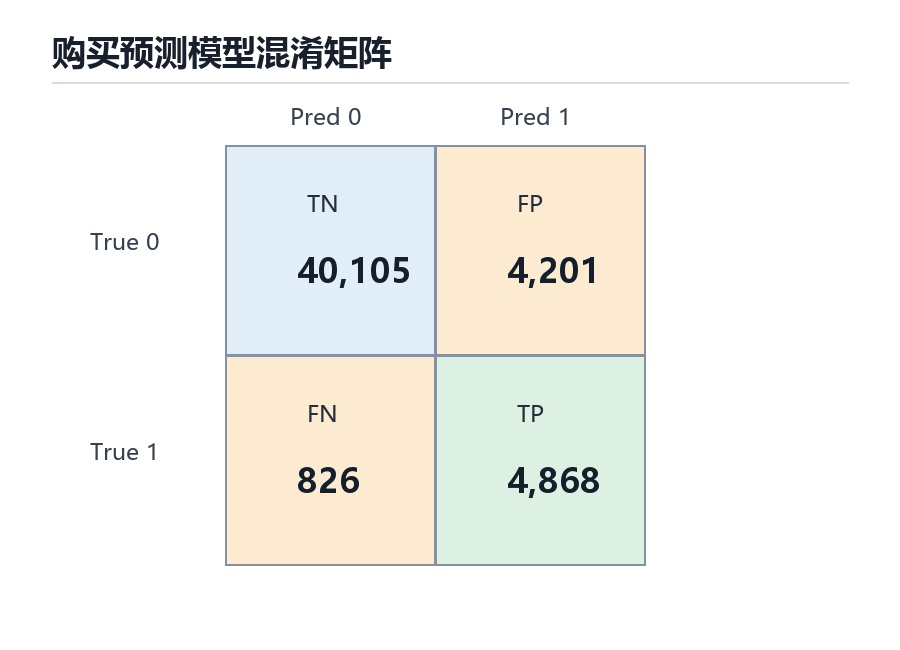
\includegraphics[width=0.70\textwidth]{model_confusion_matrix.jpg}
\caption{购买预测模型混淆矩阵}
\end{figure}

模型混淆矩阵显示，在 50,000 条测试样本中，模型识别出 4,868 个真实购买样本，同时漏判 826 个购买样本。对于电商营销场景而言，较高召回率意味着模型能够覆盖更多潜在购买用户，适合用于优惠券发放、购物车提醒和重点人群运营；精确率较低则意味着触达成本需要通过预算约束和二次排序进一步控制。

\subsection{特征解释}

特征系数结果表明，加购次数是最重要的正向变量，其次是总行为次数和会话数。这符合电商业务直觉：加购行为代表用户已经从信息浏览进入购买准备阶段，是最强的购买意图信号。浏览商品数、品类数和品牌数的系数为负，说明过度比较可能对应犹豫或尚未形成明确偏好的用户。

\begin{figure}[H]
\centering
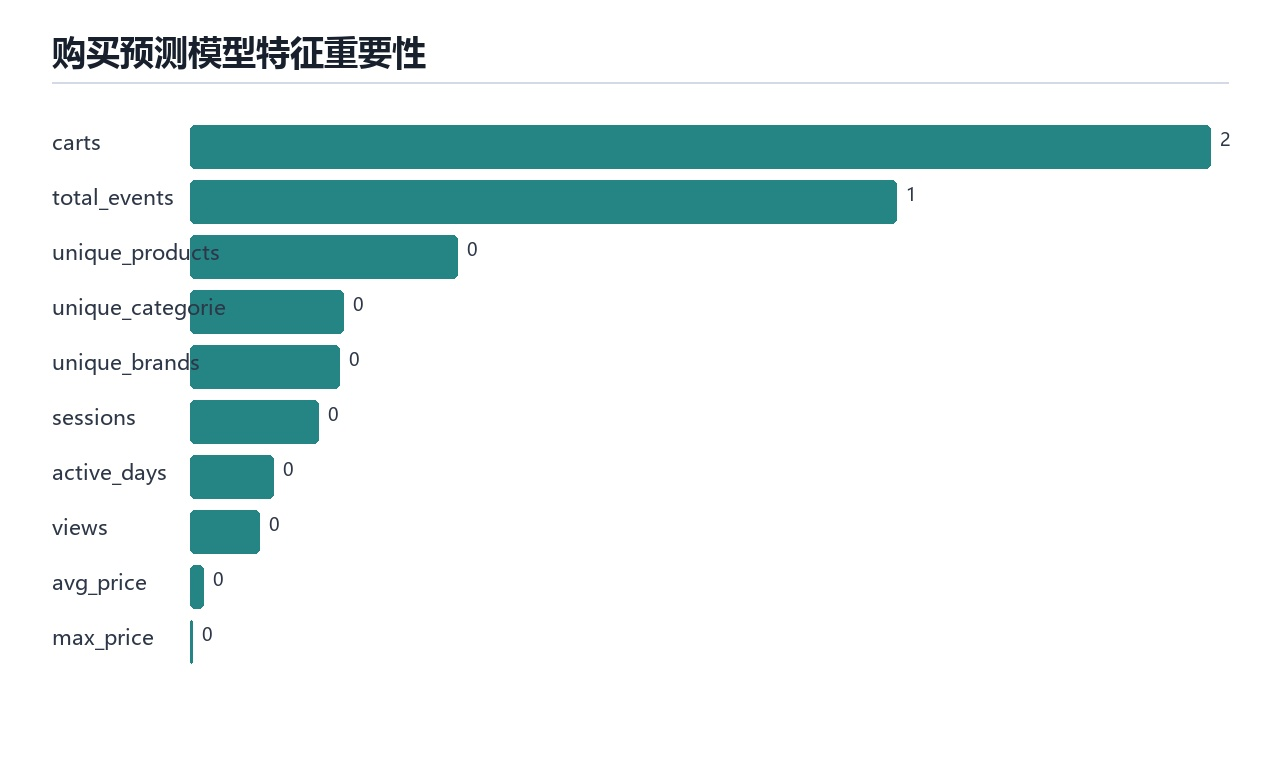
\includegraphics[width=0.90\textwidth]{model_feature_importance.jpg}
\caption{购买预测模型特征重要性}
\end{figure}

\subsection{模型结果的业务解释}

从机器学习评价指标看，模型的召回率达到 85.49\%，说明大部分真实购买用户能够被模型识别出来；精确率为 53.68\%，说明被模型判定为高意向的用户中仍有一部分最终没有购买。对于电商营销而言，这一结果是可以接受的，因为优惠券、短信、站内消息等触达成本通常低于漏掉潜在购买用户的机会成本。若平台预算较紧，可以提高分类阈值以换取更高精确率；若平台希望扩大促销覆盖面，则可以维持较低阈值以保证召回率。

从特征解释看，加购次数的系数最大，说明加购是最核心的购买意向信号。总行为次数和会话数也具有正向作用，说明活跃用户更容易转化。相反，浏览商品数、品类数和品牌数系数为负，可能意味着用户仍处在广泛比较阶段，尚未形成明确选择。这一发现可以转化为运营规则：对“加购集中但未购买”的用户进行价格提醒或优惠触达，对“浏览范围很广但未加购”的用户加强推荐排序和商品筛选，对“高客单价商品浏览用户”强化品牌和售后信息。

\section{购物车转化预测：建模深化}

\subsection{任务动机}

前一节的用户-月份模型能够识别购买倾向，但它仍然存在一个口径限制：特征和标签都来自同一个月份，因此更适合解释为用户分层，而不是严格意义上的实时预测。为了使机器学习部分更贴合数据集本身，本文进一步聚焦转化漏斗中最关键的一段，即“加购后是否购买”。

本节新增的模型称为购物车转化预测模型。其目标不是预测用户是否会在任意时间购买，而是回答：当一个用户 session 已经发生首次加购时，仅使用首次加购之前和首次加购当时可见的信息，能否判断该 session 后续是否会完成购买。这一任务与数据集中的 \texttt{view-cart-purchase} 行为链路直接对应，也更接近购物车召回、支付提醒和用户分层的业务场景。

\subsection{样本与标签定义}

新增模型以 \texttt{user\_session} 为样本单位，入样条件为 session 内至少发生一次 \texttt{cart} 事件。观察点定义为该 session 的首次加购时刻。主标签为：首次加购之后，该 session 内是否发生任意 \texttt{purchase} 事件。由于数据没有订单级明细，本文主标签采用 session 后续购买口径；同时额外计算“首次加购商品后续是否被购买”的辅助标签，用于说明同商品转化口径的扩展方向。

在工程实现上，本文仍然沿用分块读取思路，但不再只做简单聚合，而是维护一个轻量级 \texttt{session\_state} 状态字典。每个 session 只保存首次加购前累计特征、首次加购信息以及加购后是否购买，不保存原始明细。这样可以正确处理跨 chunk 的 session，同时避免将 1.77 亿条日志全部加载到内存。

\begin{lstlisting}[caption={购物车转化样本的状态更新思路}]
if state.first_cart_time is None:
    if event_type == "cart":
        state.set_first_cart(event_time, product_id, category, brand, price)
    else:
        state.update_before_cart(event_time, event_type,
                                 product_id, category, brand, price)
elif event_type == "purchase":
    state.any_purchase_after_cart = 1
    if product_id == state.first_cart_product:
        state.same_product_purchase_after_cart = 1
\end{lstlisting}

最终在 1/20 用户抽样下，本文扫描三个月全量 177,493,621 条记录，抽样处理 8,879,159 条行为，得到 216,713 个加购 session 样本。其中主标签正样本比例为 43.99\%，辅助的同商品购买比例为 41.25\%。样本构造耗时约 7.76 分钟。

\begin{table}[H]
\centering
\caption{购物车转化预测样本构造结果}
\begin{tabular}{lr}
\toprule
项目 & 数值 \\
\midrule
扫描原始记录数 & 177,493,621 \\
抽样行为记录数 & 8,879,159 \\
抽样比例 & 1/20 用户抽样 \\
加购 session 样本数 & 216,713 \\
主标签正样本比例 & 43.99\% \\
同商品购买辅助标签比例 & 41.25\% \\
样本构造耗时 & 7.76 分钟 \\
\bottomrule
\end{tabular}
\end{table}

\subsection{特征工程与训练方式}

为了避免时间泄漏，购物车转化模型只使用首次加购之前和首次加购当时可见的信息。主要特征包括首次加购前事件数、浏览数、浏览商品数、浏览品类数、浏览品牌数、首次加购商品此前被浏览次数、首次加购品类此前被浏览次数、首次加购价格、加购前平均价格、加购前最高价格、首次加购前 session 持续时间、加购小时和星期等。

训练测试划分采用跨月份方式：2019 年 10 月和 11 月样本用于训练，2019 年 12 月样本用于测试。这样可以检验模型是否能够跨月份泛化，而不是依赖随机切分带来的相似样本混合。模型仍使用 NumPy 实现的逻辑回归，另设置一个简单规则 baseline：根据首次加购前浏览强度、首次加购商品被浏览次数、是否曾浏览同商品和 session 持续时间进行排序。

\subsection{模型评估结果}

在 2019 年 12 月测试集中，共有 99,323 个加购 session，后续购买比例为 48.12\%。逻辑回归模型在分类阈值下取得 48.67\% 的精确率、97.13\% 的召回率和 0.648 的 F1 值。由于本任务的业务目标更接近“排序”而非简单二分类，本文更关注 TopK/Lift 指标，即当平台只能优先关注前 1\%、5\%、10\%、20\% 的高自然转化概率 session 时，这些 session 的真实购买率相对于随机选择提升多少。

\begin{table}[H]
\centering
\caption{购物车转化模型 TopK/Lift 结果}
\begin{tabular}{lrrrr}
\toprule
模型 & 用户池 & Precision@K & Recall@K & Lift \\
\midrule
规则 baseline & Top 10\% & 42.17\% & 8.76\% & 0.88 \\
逻辑回归 & Top 1\% & 66.67\% & 1.39\% & 1.39 \\
逻辑回归 & Top 5\% & 61.54\% & 6.39\% & 1.28 \\
逻辑回归 & Top 10\% & 60.22\% & 12.51\% & 1.25 \\
逻辑回归 & Top 20\% & 58.31\% & 24.23\% & 1.21 \\
\bottomrule
\end{tabular}
\end{table}

\begin{figure}[H]
\centering

\includegraphics[width=0.78\textwidth]{cart_conversion_lift.jpg}
\caption{购物车转化预测 Lift@K}
\end{figure}

结果表明，逻辑回归模型在高分人群排序上明显优于简单规则。以 Top 10\% 为例，模型圈出的高自然转化 session 实际购买率为 60.22\%，约为测试集平均购买率的 1.25 倍；而简单规则 baseline 的 Top 10\% Lift 低于 1，说明只靠浏览强度和简单同商品信号并不能有效识别自然转化用户。

\begin{figure}[H]
\centering
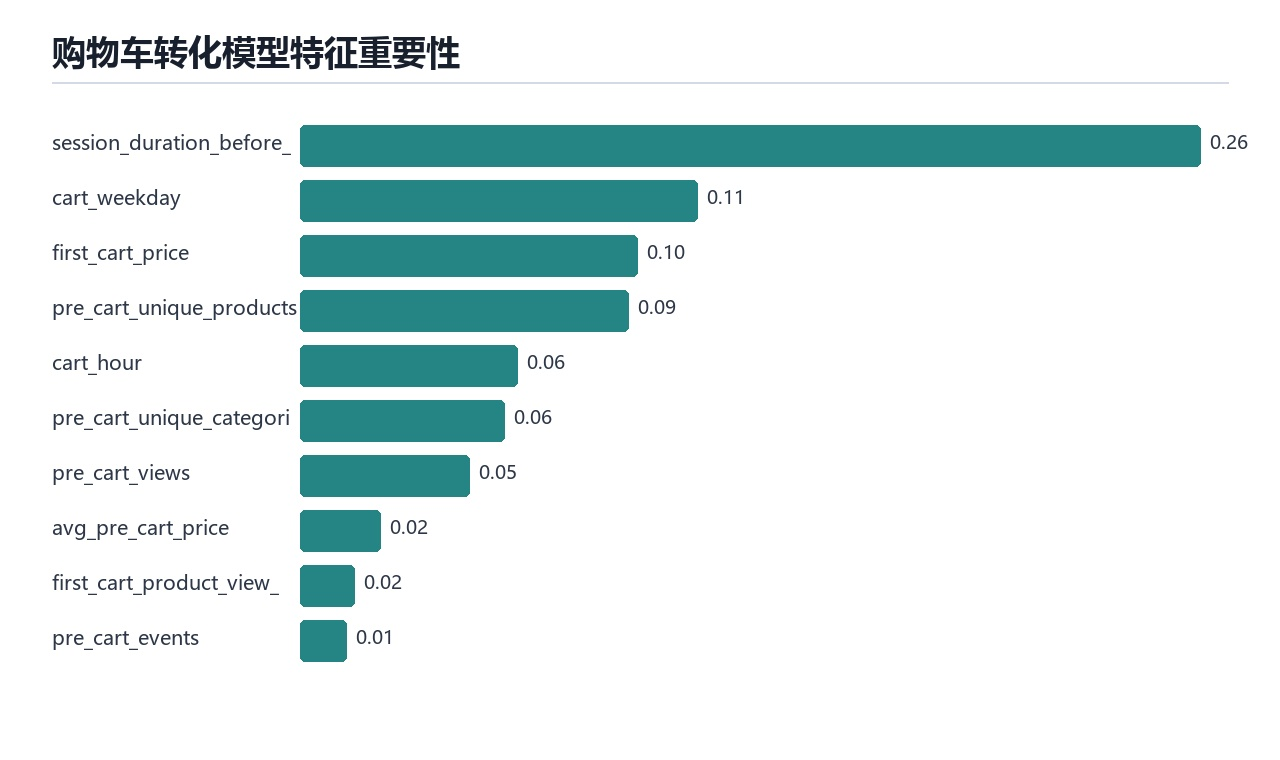
\includegraphics[width=0.88\textwidth]{cart_conversion_feature_importance.jpg}
\caption{购物车转化模型特征重要性}
\end{figure}

特征结果显示，首次加购前 session 持续时间、首次加购价格、浏览商品范围、加购小时和首次加购商品此前浏览次数等变量对模型排序具有较大影响。与前一节月度购买倾向模型相比，购物车转化模型的解释粒度更细：它不再只判断用户是否活跃，而是判断用户在一个具体 session 中是否已经形成足够明确的购买意图。

\subsection{业务解释边界}

需要注意，高预测分数表示该 session 更可能自然完成购买，并不等于最需要发券召回。对于高自然转化概率用户，平台可以减少过度优惠，更多使用库存提醒、支付提醒和服务保障信息；对于低自然转化概率但首次加购价格较高的 session，则更接近潜在流失且值得干预的人群。本文据此构造了一个辅助人群：首次加购价格高于测试集中位数、自然转化概率处于最低 20\% 的 session，共 5,545 个，平均首次加购价格为 372.41，实际购买率为 40.79\%。这类用户不一定会自然转化，但商品价值较高，适合作为购物车召回候选池。

因此，本模型的合理用途不是替代业务决策，而是给购物车用户分层提供排序依据：高自然转化概率人群用于识别强意向用户，低自然转化但高价值人群用于识别召回候选。由于数据集中没有优惠券、活动曝光、库存和物流字段，本文不将该模型解释为促销因果分析或推荐系统。

\section{结论与建议}

本文基于三个月、1.77 亿条电商行为日志，完成了从数据读取、清洗聚合、描述统计、漏斗分析到机器学习预测的完整分析流程。主要结论如下：

\begin{enumerate}
  \item 用户行为呈现典型漏斗结构，浏览事件远高于加购和购买事件，平台转化提升的重点在于减少浏览到加购、加购到支付之间的流失。
  \item 11 月和 12 月的行为规模明显高于 10 月，但促销期流量增长并不必然等同于转化效率提升，需要同时监控购物车转化率和支付完成率。
  \item 消费电子类商品贡献了主要销售额，手机、灯具、耳机、电视和家电品类具有较高经营价值；Apple 和 Samsung 等品牌分别体现了高客单价和高交易频次特征。
  \item 用户-月份模型能够识别整体购买倾向，加购次数、总行为次数和会话数是关键预测变量，可用于用户分层和精准营销。
  \item 购物车转化模型进一步聚焦首次加购后的 session 转化，逻辑回归在 12 月测试集 Top 10\% 人群中达到 60.22\% 的真实购买率，Lift 为 1.25，可用于购物车用户排序。
\end{enumerate}

基于上述结论，本文提出以下运营建议：第一，对加购未购买用户建立重点触达机制，结合库存提醒、支付提醒和必要的价格策略降低流失；第二，在促销月区分流量增长和转化增长，避免只关注浏览峰值；第三，对高销售额品类进行更精细的价格带和品牌结构管理；第四，将购买预测模型作为营销排序工具，而不是机械替代业务判断。对于高自然转化概率用户，应避免无差别发券；对于低自然转化但高商品价值的用户，可以优先进入购物车召回候选池。

\section{课程技术应用闭环}

本案例与课程内容的对应关系较为完整。首先，在数据获取层面，本文使用公开数据集替代实时爬虫，原因是期末作业更关注可复现的大数据分析流程，而该数据集已经具备真实平台日志的规模和字段结构。其次，在数据处理层面，本文使用 Python、Pandas 和 NumPy 处理压缩 CSV，并采用分块计算避免一次性加载亿级数据。再次，在分析层面，本文从事件、时间、品类、品牌和价格多个维度进行统计，体现经济数据分析中常见的分组、聚合和比较方法。最后，在机器学习层面，本文使用逻辑回归完成购买倾向识别和购物车转化排序，并通过混淆矩阵、精确率、召回率、F1 值以及 TopK/Lift 指标评价模型。

从“问题--数据--方法--结论--建议”的链条看，本文不是单纯堆砌技术。研究问题来自电商平台转化效率；数据来自用户行为日志；方法包括分块处理、漏斗分析和分类模型；结论回到用户流失、商品结构和运营触达。这样的闭环能够体现大数据分析在经济管理场景中的实际价值。

\begin{table}[H]
\centering
\caption{课程技术与本文实现的对应关系}
\begin{tabular}{p{0.24\textwidth}p{0.28\textwidth}p{0.38\textwidth}}
\toprule
课程技术点 & 本文实现 & 对应作用 \\
\midrule
Python 基础与脚本化处理 & 统一脚本读取、清洗、聚合、输出图表 & 保证流程可复现 \\
Pandas 数据分析 & 分块读取、分组统计、透视表、特征聚合 & 支撑亿级事件日志处理 \\
NumPy 数值计算 & 逻辑回归、矩阵计算、指标计算 & 实现机器学习模型 \\
数据可视化 & 行为量、漏斗、品类、品牌、模型结果图 & 将统计结论转化为可解释图表 \\
机器学习方法 & 用户购买倾向识别、购物车转化排序 & 支持潜在购买用户识别和加购 session 分层 \\
\bottomrule
\end{tabular}
\end{table}

\section{不足与展望}

本文仍存在若干不足。首先，唯一用户漏斗采用确定性抽样估计，虽然适合在本地环境下控制内存，但相比全量去重仍存在抽样误差。其次，初步用户-月份模型的标签使用月度购买结果，尚未严格区分购买前行为和购买后行为；后续的购物车转化模型虽然改为首次加购前后口径，但仍局限于 session 内行为，无法观察优惠券、库存、物流和真实触达等变量。最后，本文使用逻辑回归模型以保证可解释性，未来可以进一步尝试树模型、梯度提升模型或序列模型，以提升非线性关系捕捉能力。

总体而言，本案例展示了 Python 在经济大数据分析中的完整应用路径：面对压缩大文件，通过分块读取和聚合降低内存压力；面对复杂行为数据，通过特征工程形成可建模样本；面对业务问题，通过漏斗分析和机器学习模型将数据结果转化为运营解释。

需要强调的是，本文没有将模型结果解释为因果关系。例如，加购次数与购买概率高度相关，并不意味着单纯提高加购次数就一定会导致购买增加；它更合理的解释是用户购买意图增强的行为表现。后续若要研究促销、推荐或价格变化对购买的因果影响，还需要引入实验设计、倾向得分匹配或双重差分等方法。

%%----------- 参考文献 -------------------%%
\begin{thebibliography}{9}
\bibitem{kaggle}
Kechinov M. E-commerce behavior data from multi category store. Kaggle Dataset. \url{https://www.kaggle.com/datasets/mkechinov/ecommerce-behavior-data-from-multi-category-store}.
\bibitem{pandas}
The pandas development team. pandas: powerful Python data analysis toolkit. \url{https://pandas.pydata.org/}.
\bibitem{numpy}
Harris C. R. et al. Array programming with NumPy. Nature, 585, 357--362, 2020.
\end{thebibliography}

\end{document}
